% ============================================================================
% Method — DUET
% ============================================================================

\section{DUET: Dual-Channel Teacher Utilization}
\label{sec:method}

\subsection{Setup}
\label{sec:setup}

We train a student policy $\pi_\theta(a\mid s)$ with GRPO~\citep{shao2024deepseekmath} in sparse-reward interactive environments.
For each task, the student samples $n_o$ on-policy rollouts $G^o$.
We also use a fixed cache of successful trajectories $\{\tau^\beta\}$ collected from a stronger teacher policy $\pi_\beta$.
Following teacher-mixed replay~\citep{yan2025luffy, zhang2025chord}, each training group includes $n_\beta$ teacher trajectories $G^\beta$:
\begin{equation}
G = G^o \cup G^\beta,
\qquad
|G| = n_o+n_\beta .
\label{eq:mixed_group}
\end{equation}
Our goal is to use this cache without letting off-policy teacher trajectories distort the group-normalized policy-gradient update.

\subsection{Overview}
\label{sec:overview}

\begin{figure}[t]
\centering
\IfFileExists{figures/fig1_method.pdf}{%
  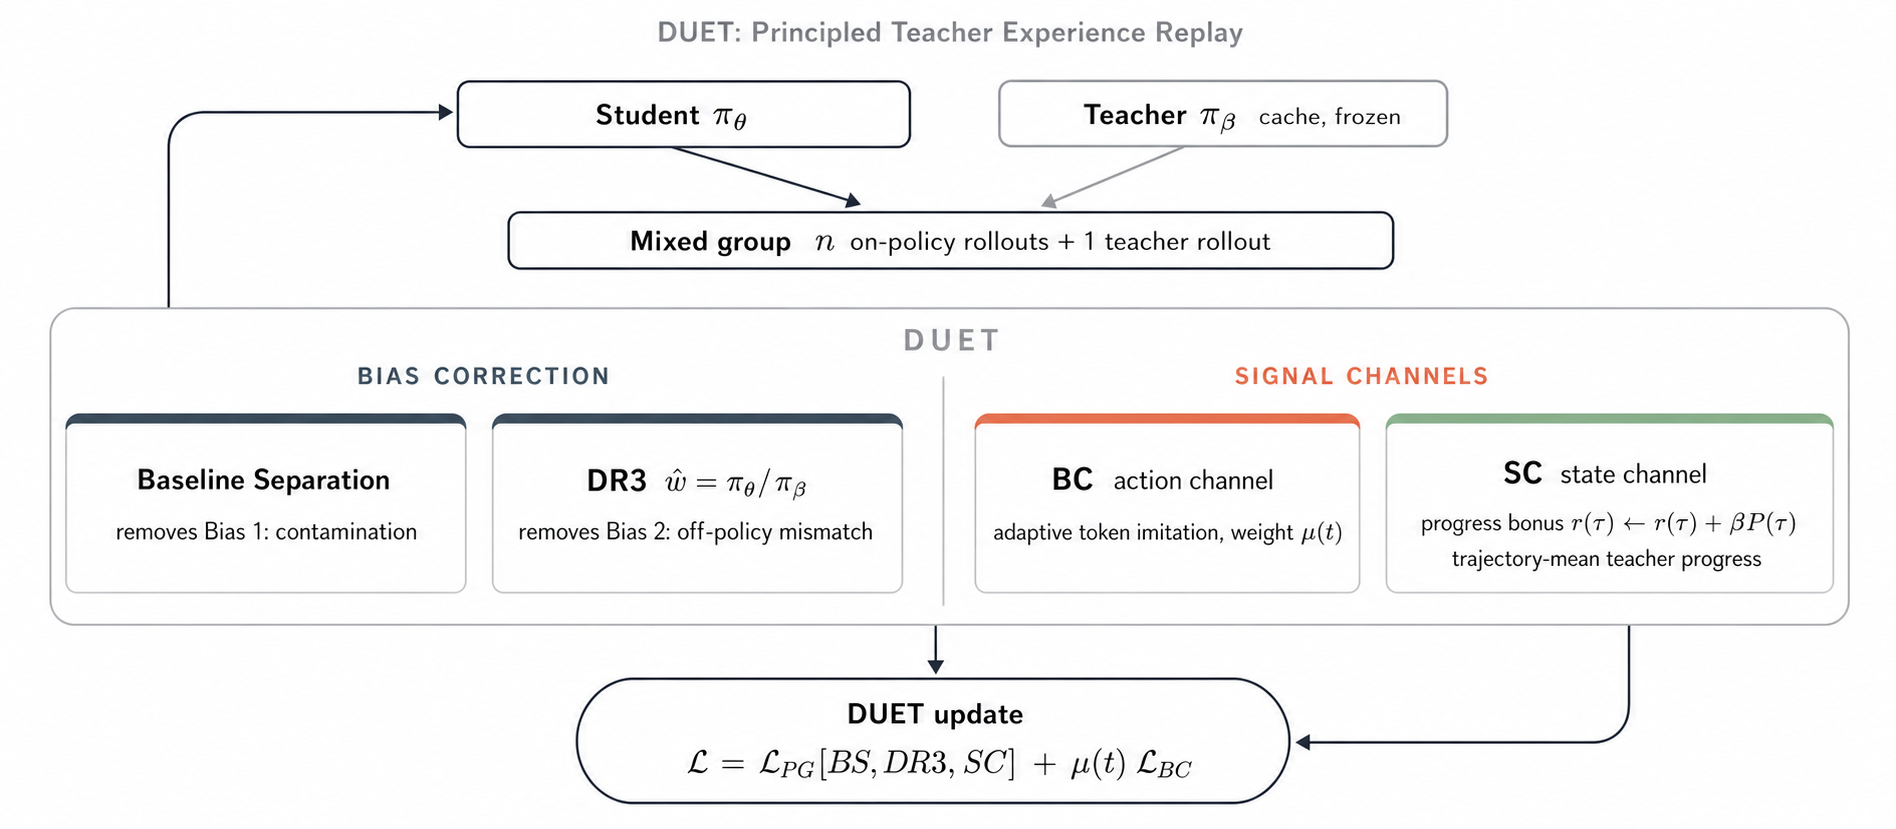
\includegraphics[width=0.95\linewidth]{figures/fig1_method.pdf}%
}{\IfFileExists{figures/fig1_method.png}{%
  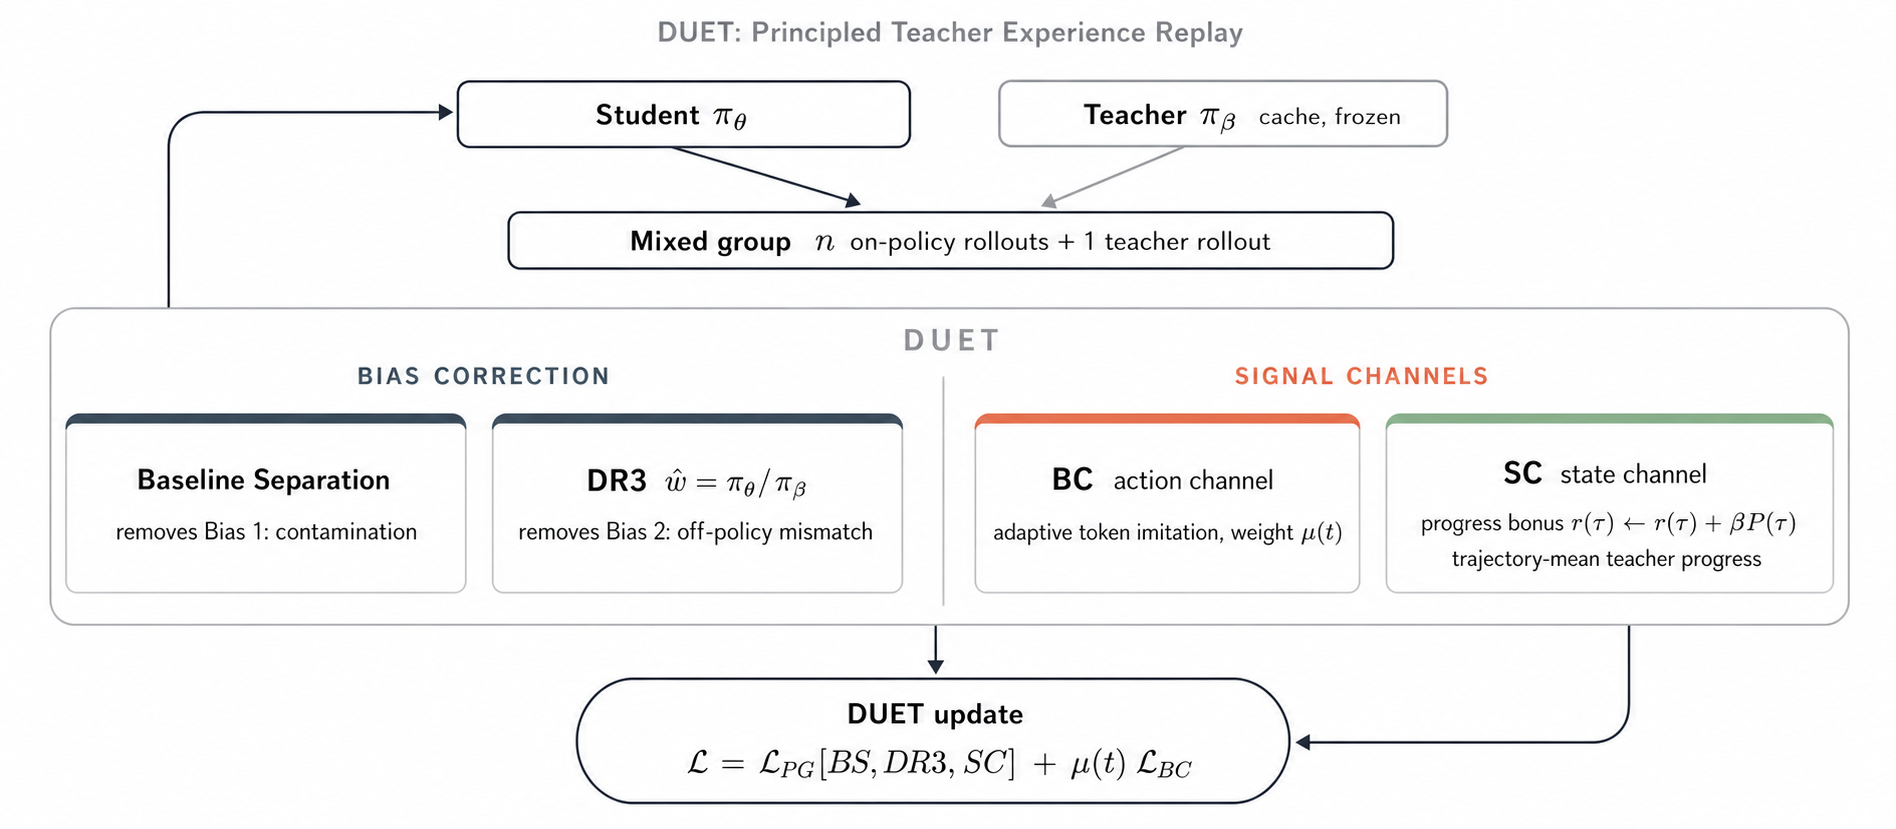
\includegraphics[width=0.95\linewidth]{figures/fig1_method.png}%
}{\IfFileExists{figures/fig1_method.jpg}{%
  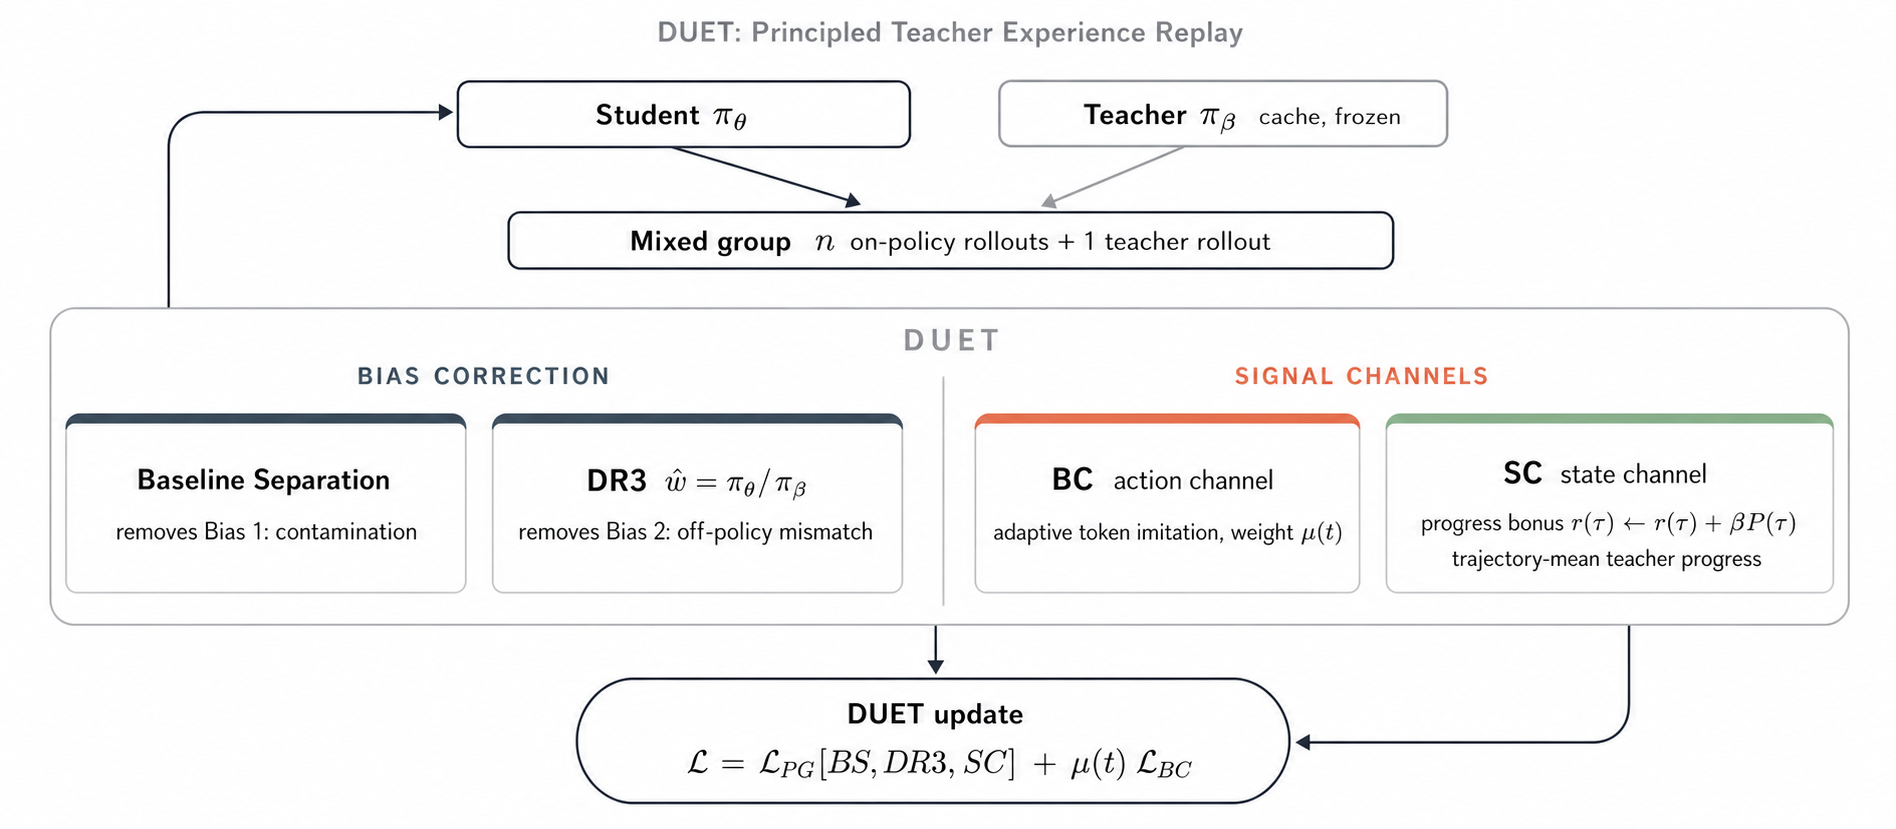
\includegraphics[width=0.95\linewidth]{figures/fig1_method.jpg}%
}{%
  \fbox{\parbox{0.9\linewidth}{\centering\vspace{4em}\itshape Figure~1 placeholder --- DUET architecture diagram.\vspace{4em}}}%
}}}
\caption{
\textbf{DUET overview.}
Teacher trajectories provide both action-level and state-level information.
The Action Channel uses teacher actions with baseline separation and density-ratio correction.
The State Channel uses teacher observations to construct a progress map and shape rewards for on-policy rollouts.
}
\label{fig:method}
\end{figure}

DUET uses teacher trajectories through two complementary channels.
The \textbf{Action Channel} determines how teacher actions enter the policy update: it separates teacher and on-policy baselines, estimates a teacher--student density ratio when exact importance correction is unavailable, and adds behavior cloning as a cold-start bridge.
The \textbf{State Channel} uses teacher observations to estimate task progress and shape rewards for on-policy rollouts.
Thus, teacher actions provide corrected action-level supervision, while teacher states provide progress-based exploration guidance.

\subsection{Action Channel}
\label{sec:action_channel}

\paragraph{Baseline contamination.}
In teacher-mixed GRPO, successful teacher trajectories can raise the group baseline and suppress credit assigned to on-policy rollouts.
Let $p_o$ be the on-policy success rate in a group, and assume replayed teacher trajectories are successful, $R^\beta=1$.
The pooled reward mean is
\begin{equation}
\mu_{\mathrm{pool}}
=
\frac{n_o p_o+n_\beta}{n_o+n_\beta}.
\label{eq:pooled_mean}
\end{equation}
Under this pooled baseline, the expected centered reward of an on-policy rollout is
\begin{equation}
\mathbb{E}_{i\in G^o}
\left[
R^{o,(i)}-\mu_{\mathrm{pool}}
\right]
=
p_o-\frac{n_o p_o+n_\beta}{n_o+n_\beta}
=
-\frac{n_\beta}{n_o+n_\beta}(1-p_o).
\label{eq:baseline_contamination}
\end{equation}
Thus, whenever $p_o<1$, pooled normalization introduces a negative shift for on-policy samples.
The shift is largest during cold start, but persists until the student succeeds on nearly all rollouts.
It therefore suppresses the rare exploratory successes that RL should amplify.

\paragraph{Asymmetric baseline separation.}
DUET removes this shift by centering on-policy samples only against the on-policy subgroup:
\begin{equation}
\hat A^{o,(i)}
=
\frac{R^{o,(i)}-\mu^o}{\sigma^o},
\qquad
\mu^o=
\frac{1}{|G^o|}
\sum_{j\in G^o}R^{o,(j)} ,
\label{eq:on_policy_advantage}
\end{equation}
where $\sigma^o$ is the standard deviation of on-policy rewards.
Teacher samples are centered against the pooled mean and scaled by the same on-policy standard deviation:
\begin{equation}
\hat A^{\beta,(i)}
=
\frac{R^{\beta,(i)}-\mu_{\mathrm{pool}}}{\sigma^o}.
\label{eq:teacher_advantage}
\end{equation}
This asymmetric rule keeps on-policy advantages centered within $G^o$, while giving successful teacher samples positive advantage when the student is weak:
\begin{equation}
R^{\beta,(i)}-\mu_{\mathrm{pool}}
=
1-\mu_{\mathrm{pool}}
=
\frac{n_o}{n_o+n_\beta}(1-p_o).
\label{eq:teacher_centered_reward}
\end{equation}
As the student improves, the teacher advantage naturally decreases.
Using $\sigma^o$ also avoids the zero-variance issue of success-filtered teacher batches.

\paragraph{Density-Ratio Repair (DR3).}
We refer to the missing teacher--student correction as a \emph{repair} on the standard policy ratio, and abbreviate the resulting estimator as DR3.
Teacher actions are generated by $\pi_\beta$, while the standard GRPO ratio
\begin{equation}
\rho_t
=
\frac{\pi_\theta(a_t\mid s_t)}
{\pi_{\theta_{\mathrm{old}}}(a_t\mid s_t)}
\label{eq:grpo_ratio}
\end{equation}
only accounts for the change from the old student policy to the current one.
When teacher log-probabilities are unavailable, DUET estimates the missing teacher--student ratio with a discriminator $D_\phi(s,a)$ trained to distinguish on-policy from teacher state--action pairs:
\begin{equation}
\hat w(s,a)
=
\frac{D_\phi(s,a)}{1-D_\phi(s,a)}
\approx
\frac{\pi_\theta(a\mid s)}
{\pi_\beta(a\mid s)} .
\label{eq:dr3_ratio}
\end{equation}
$D_\phi$ is a lightweight MLP over sequence-level features and outputs the probability that $(s,a)$ comes from the on-policy student rather than the teacher cache.
It is updated jointly with the actor at every policy step from a rolling buffer of recent on-policy and teacher samples, so $\hat w$ tracks the evolving student distribution rather than a fixed snapshot.
The feature set and training procedure are detailed in Appendix~\ref{app:disc}.
This gives the corrected teacher replay term
\begin{equation}
\mathcal{L}_{\mathrm{PG}}^{\mathrm{tch}}(\theta)
=
-\mathbb{E}_{(s,a)\sim G^\beta}
\left[
\hat A^\beta
\cdot
\mathrm{clip}
\left(
\hat w(s,a)\rho_t,
1-\varepsilon,
1+\varepsilon
\right)
\right].
\label{eq:dr3_loss}
\end{equation}
We use $\hat w$ as a bias-mitigating replay weight rather than an exact likelihood ratio, since the teacher cache is success-filtered.
It also attenuates teacher gradients according to the estimated teacher--student distribution gap, instead of a fixed training-step schedule.

\paragraph{Adaptive behavior cloning.}
Early in training, the discriminator has limited data, so DUET adds token-level behavior cloning on teacher trajectories:
\begin{equation}
\mathcal{L}_{\mathrm{BC}}(\theta)
=
-\mathbb{E}_{(s,a)\sim G^\beta}
\left[
\log \pi_\theta(a\mid s)
\right].
\label{eq:bc_loss}
\end{equation}
Its coefficient $\mu(t)$ is high during cold start and decays as the discriminator becomes informative.
This provides dense action supervision before the density-ratio correction stabilizes.
Implementation details are in Appendix~\ref{app:impl}.

\subsection{State Channel}
\label{sec:state_channel}

The State Channel extracts progress information from states visited by successful teacher trajectories.
For each teacher trajectory $\tau^\beta=(s_0^\beta,\ldots,s_{T_{\tau^\beta}}^\beta)$, we assign every observation a within-trajectory progress value $\phi(s_t^\beta;\tau^\beta)=t/T_{\tau^\beta}$.
We then aggregate these values across the teacher cache into a state potential
\begin{equation}
\Phi(s)
=
\frac{1}{|\mathcal{T}_\beta(s)|}
\sum_{(\tau^\beta,t)\in\mathcal{T}_\beta(s)}
\phi(s_t^\beta;\tau^\beta),
\qquad
\Phi:\mathcal{S}\to[0,1],
\label{eq:progress_potential}
\end{equation}
where $\mathcal{T}_\beta(s)=\{(\tau^\beta,t):s_t^\beta=s\}$ is the set of all teacher visits to state $s$, and unmatched states are assigned $\Phi(s)=0$.
For an on-policy trajectory $\tau=(s_0,a_0,\ldots,s_T)$, DUET computes
\begin{equation}
P(\tau)
=
\frac{1}{T+1}
\sum_{t=0}^{T}\Phi(s_t),
\qquad
r'(\tau)
=
r(\tau)+\lambda P(\tau).
\label{eq:sc_shaping}
\end{equation}
Here $r(\tau)$ is the environment task reward and $\lambda>0$ is the shaping coefficient (chosen as a small constant to avoid overwhelming the task reward).
This trajectory-level shaping gives dense feedback when environment rewards are sparse.
It is inspired by potential-based reward shaping~\citep{ng1999policy}, but we use an empirical trajectory-level score and do not claim exact policy invariance.
The bonus is applied only to on-policy rollouts; teacher trajectories keep their original rewards.

\subsection{Combined objective}
\label{sec:duet_update}

The DUET loss combines shaped on-policy RL, corrected teacher replay, and cold-start behavior cloning:
\begin{equation}
\mathcal{L}_{\mathrm{DUET}}(\theta)
=
\sum_{i\in G^o}
\mathcal{L}_{\mathrm{PG}}^{\mathrm{on}}
\left(
\hat A_{\mathrm{shaped}}^{o,(i)};\theta
\right)
+
\sum_{j\in G^\beta}
\mathcal{L}_{\mathrm{PG}}^{\mathrm{tch}}
\left(
\hat A^{\beta,(j)},\hat w^{(j)};\theta
\right)
+
\mu(t)\mathcal{L}_{\mathrm{BC}}(\theta).
\label{eq:duet_full_loss}
\end{equation}
$\hat A_{\mathrm{shaped}}^{o}$ is obtained by substituting the shaped reward $r'(\tau)$ from Eq.~\eqref{eq:sc_shaping} for $R^{o,(i)}$ in the on-policy advantage formula Eq.~\eqref{eq:on_policy_advantage}; teacher samples use $\hat A^\beta$ from Eq.~\eqref{eq:teacher_advantage} together with the density-ratio weight $\hat w$ from Eq.~\eqref{eq:dr3_ratio}.